\section{Solución}

\subsection{Descripción}
Como se mencionó anteriormente se espera \textbf{una escalabilidad horizontal} y
principalmente una \textbf{alta disponibilidad (99.5\%)}, además de esto el
cliente requiere de desplegarlo en \textit{AWS}. \\

Por lanto, decidimos usar un \textit{balanceador de cargas clásico} de
\textit{AWS} para desplegar los \textit{EC2} (Una instancia virtual de un
servidor de Amazon) requeridos por la organización. Por lo que decidimos
desplegar la siguiente arquitectura:

\begin{figure}[H]
    \centering
    \begin{subfigure}[b]{0.8\textwidth}
        \centering
        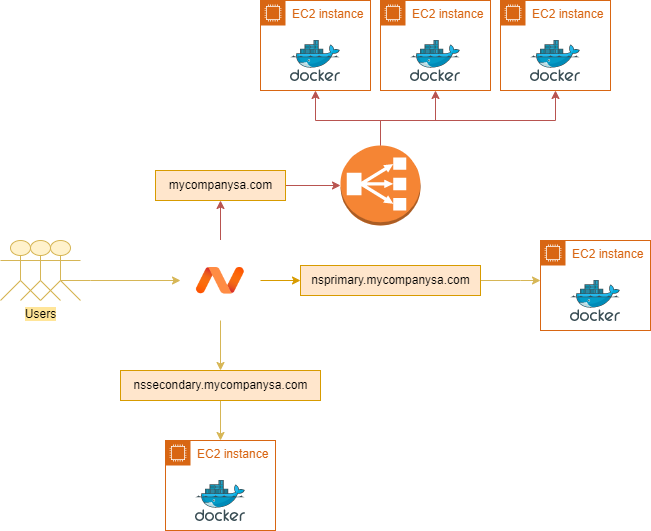
\includegraphics[width=\textwidth]{Figures/0. General/mycompanysa_architecture.png}
        \caption{\textit{Arquitectura de mycompanysa}}
        \label{fig: mycompanysa architecture}
    \end{subfigure}
\end{figure}

\subsection{Configuración}
En el siguiente apartado se documentará el proceso de cómo se hizo, esto ya sea
para una replica del proceso a futuros proyectos o para la mejora del mismo 
proyecto. \\

\subsubsection{Creación de Load Balancer con 3 instancias en AWS}
Primero debemos entrar en ec2 y crear una nueva instancia en "Lanzar instancia"

\begin{figure}[H]
    \centering
    \begin{subfigure}[b]{0.8\textwidth}
        \centering
        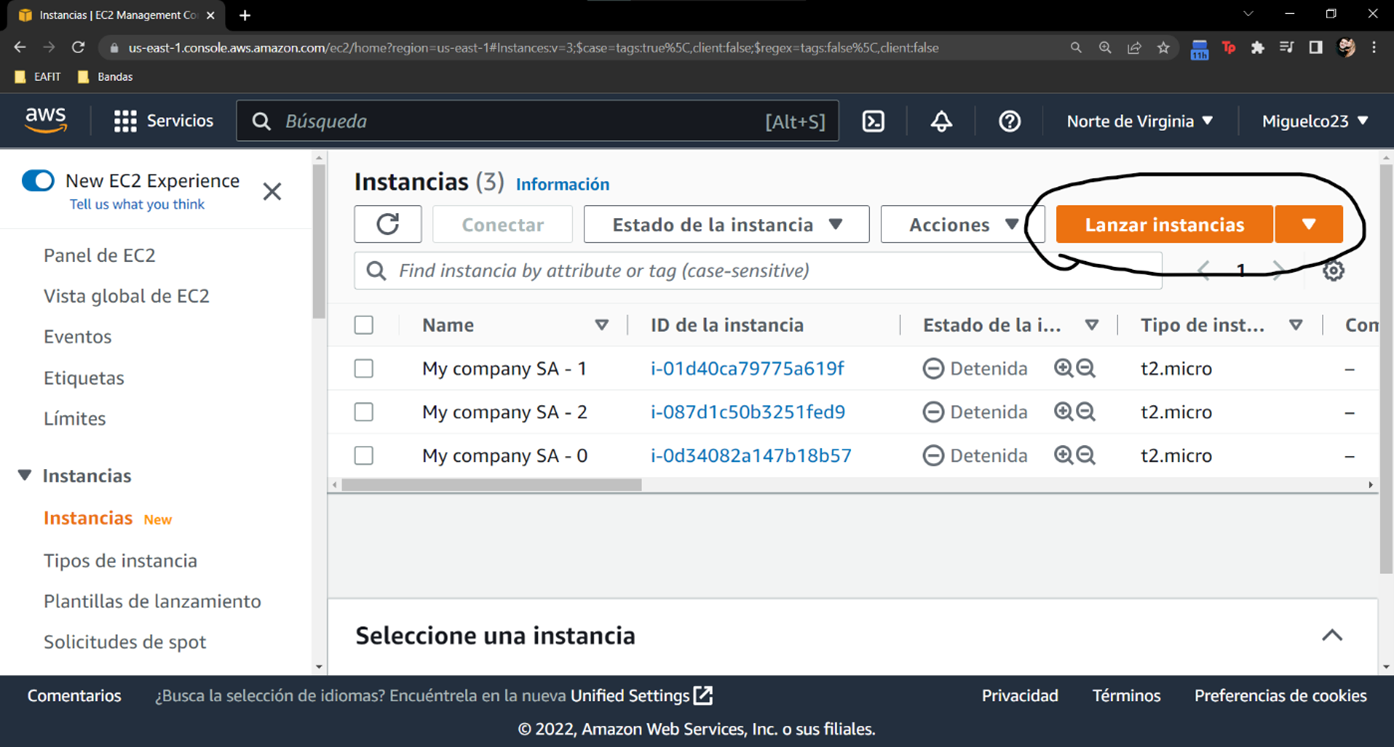
\includegraphics[width=\textwidth]{Figures/0. General/load_balancer_0.png}
        \caption{\textit{Creamos una nueva instancia}}
        \label{fig: load balancer 0}
    \end{subfigure}
\end{figure}

En el área de configuraciones de \textit{red/grupos} de seguridad debemos
activar el tráfico a través de \textit{HTTP}.

\begin{figure}[H]
    \centering
    \begin{subfigure}[b]{0.8\textwidth}
        \centering
        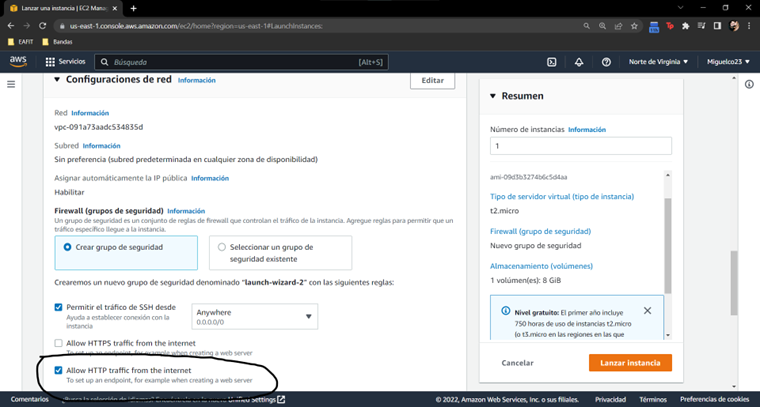
\includegraphics[width=\textwidth]{Figures/0. General/load_balancer_1.png}
        \caption{\textit{Configuraciones de \textit{red/grupos} de seguridad}}
        \label{fig: load balancer 1}
    \end{subfigure}
\end{figure}

Además, agregamos nuestra llave (Key par) para acceder a la instancia remotamente.

\begin{figure}[H]
    \centering
    \begin{subfigure}[b]{0.8\textwidth}
        \centering
        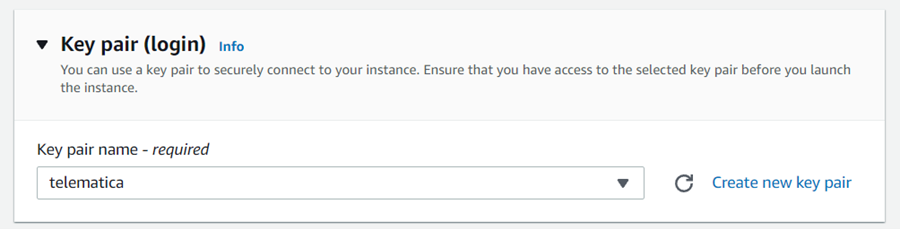
\includegraphics[width=\textwidth]{Figures/0. General/load_balancer_2.png}
        \caption{\textit{Opciones Key Par}}
        \label{fig: load balancer 2}
    \end{subfigure}
\end{figure}

En este caso (Aunque no es estrictamente necesario para crear el balanceador)
pondremos un script en la sección de datos de usuario, para así ver a cuál
instancia en específico estamos accediendo. Despues de esto lanzamos la instancia.

\begin{lstlisting}[language=Bash]
#!/bin/bash
yum update -y
yum install -y httpd.x86_64
systemctl start httpd.service
systemctl enable httpd.service
echo "Hola Mundo desde $(hostname -f)" > /var/www/html/index.html
\end{lstlisting}

\begin{figure}[H]
    \centering
    \begin{subfigure}[b]{0.8\textwidth}
        \centering
        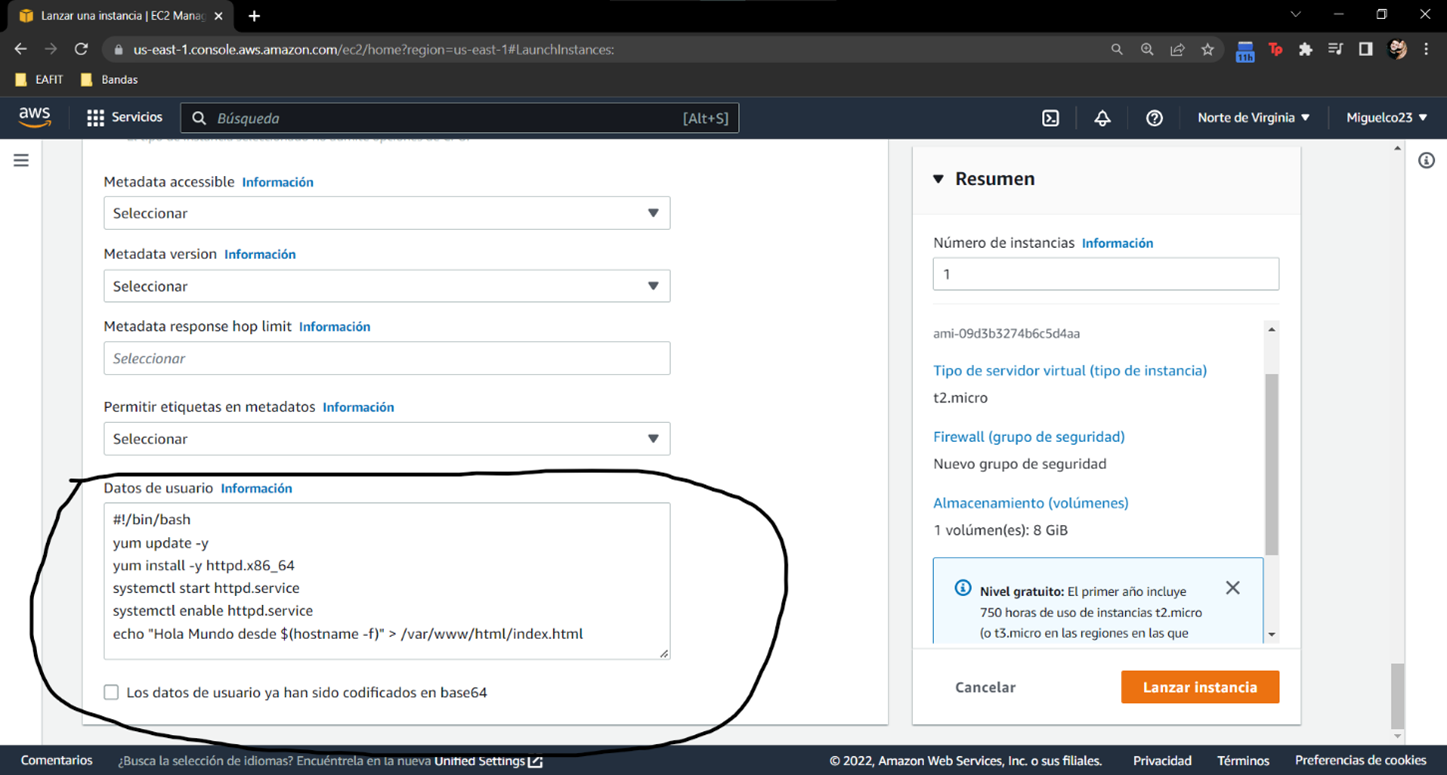
\includegraphics[width=\textwidth]{Figures/0. General/load_balancer_3.png}
        \caption{\textit{Script de configuración inicial}}
        \label{fig: load balancer 3}
    \end{subfigure}
\end{figure}

Al tener nuestra instancia, damos clic derecho en ella:
\textbf{\textit{imagen y plantillas/lanzar más como esta}}. Para así duplicarla
(En este casi lo hicimos dos veces para tener 3 instancias diferentes).

\begin{figure}[H]
    \centering
    \begin{subfigure}[b]{0.8\textwidth}
        \centering
        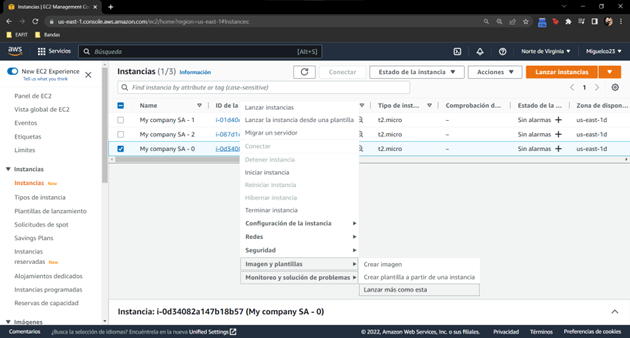
\includegraphics[width=\textwidth]{Figures/0. General/load_balancer_4.png}
        \caption{\textit{Imagen y plantillas}}
        \label{fig: load balancer 4}
    \end{subfigure}
\end{figure}

Para continuar buscamos en el panel de EC2:
\textbf{\textit{equilibrio de carga/balanceadores de carga}} y entramos.

\begin{figure}[H]
    \centering
    \begin{subfigure}[b]{0.8\textwidth}
        \centering
        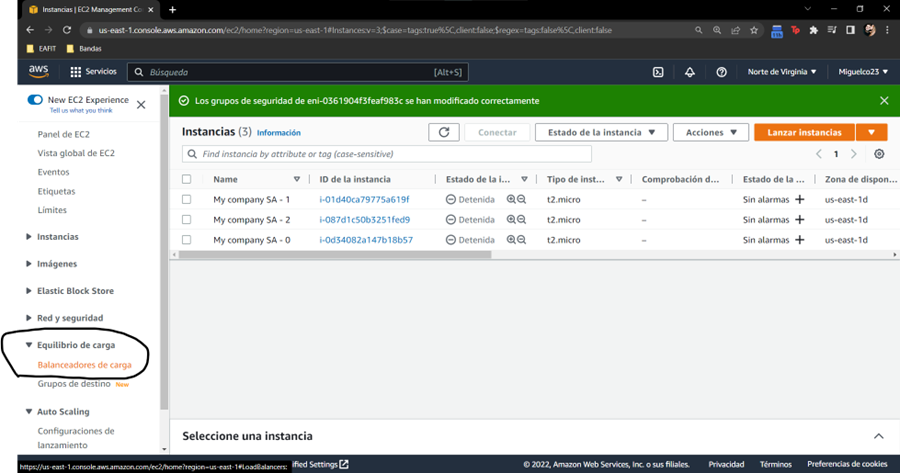
\includegraphics[width=\textwidth]{Figures/0. General/load_balancer_5.png}
        \caption{\textit{Equilibrio de cargas}}
        \label{fig: load balancer 5}
    \end{subfigure}
\end{figure}

Damos click en \textbf{\textit{Crear balanceador de carga}}:

\begin{figure}[H]
    \centering
    \begin{subfigure}[b]{0.8\textwidth}
        \centering
        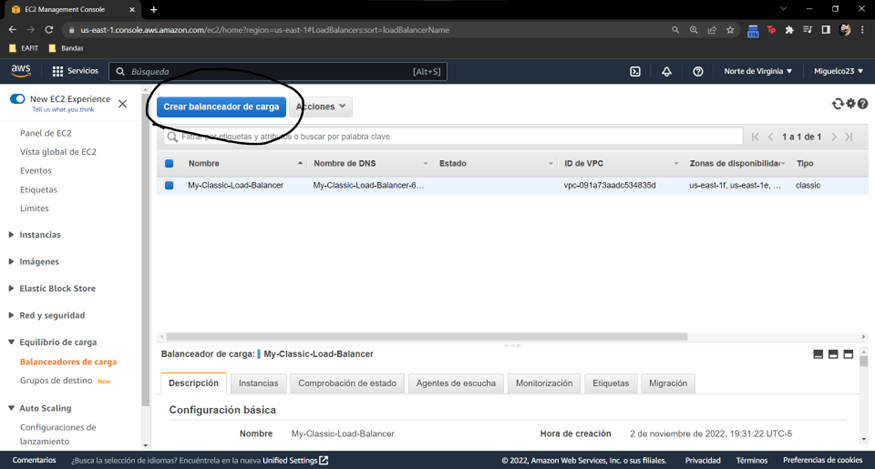
\includegraphics[width=\textwidth]{Figures/0. General/load_balancer_6.png}
        \caption{\textit{Click en balanceador de cargas}}
        \label{fig: load balancer 6}
    \end{subfigure}
\end{figure}

Seleccionamos \textbf{\textit{Classic load balancer}}.

\begin{figure}[H]
    \centering
    \begin{subfigure}[b]{0.8\textwidth}
        \centering
        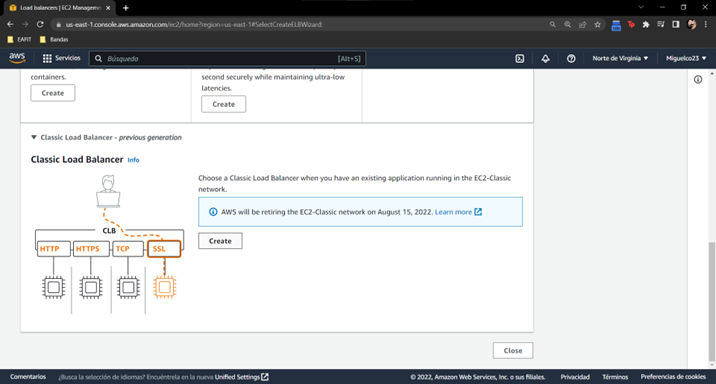
\includegraphics[width=\textwidth]{Figures/0. General/load_balancer_7.png}
        \caption{\textit{Click en Classic load balancer}}
        \label{fig: load balancer 7}
    \end{subfigure}
\end{figure}

En el paso de \textbf{\textit{"Asignar grupos de seguridad"}} creamos un nuevo
grupo con una regla de tipo HTTP y origen cualquier lugar.

\begin{figure}[H]
    \centering
    \begin{subfigure}[b]{0.8\textwidth}
        \centering
        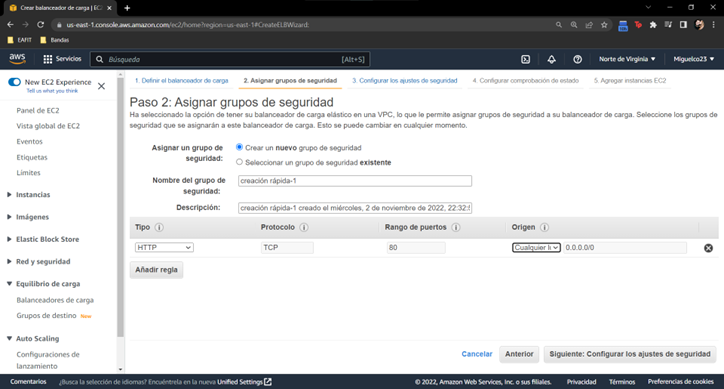
\includegraphics[width=\textwidth]{Figures/0. General/load_balancer_8.png}
        \caption{\textit{Click en Asignar grupos de seguridad}}
        \label{fig: load balancer 8}
    \end{subfigure}
\end{figure}

En el paso siguiente agregamos las instancias que creamos previamente y que queremos que
hagan parte del balanceador.

\begin{figure}[H]
    \centering
    \begin{subfigure}[b]{0.8\textwidth}
        \centering
        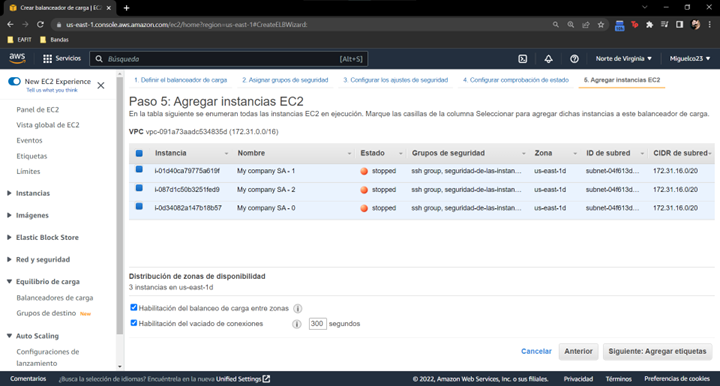
\includegraphics[width=\textwidth]{Figures/0. General/load_balancer_9.png}
        \caption{\textit{Agregar las instancias}}
        \label{fig: load balancer 9}
    \end{subfigure}
\end{figure}

Una vez que nuestro balanceador esté listo, a al darle clic, podremos ver debajo
el nombre del DNS para acceder a este.

\begin{figure}[H]
    \centering
    \begin{subfigure}[b]{0.8\textwidth}
        \centering
        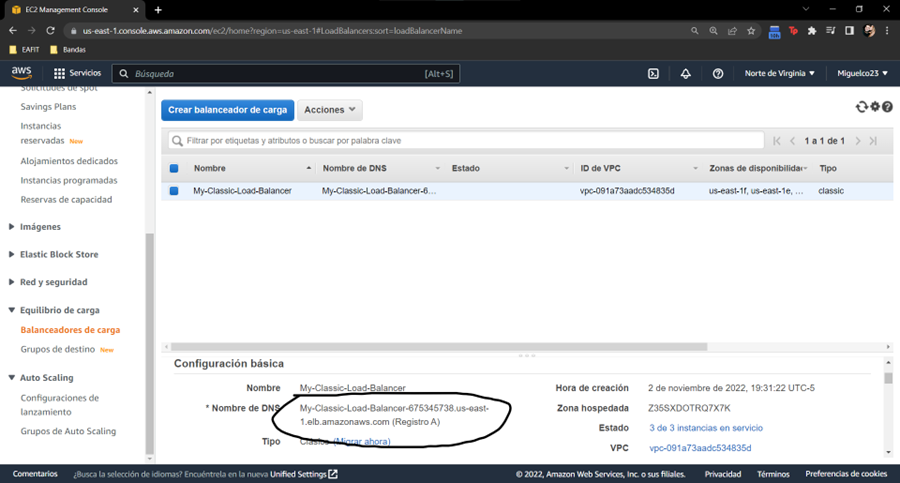
\includegraphics[width=\textwidth]{Figures/0. General/load_balancer_10.png}
        \caption{\textit{Revisamos las instancias}}
        \label{fig: load balancer 10}
    \end{subfigure}
\end{figure}

Al ingresar a nuestro DNS e ir actualizando podemos ver como desde el mismo URL
accedemos a las diferentes instancias. Por lo que está funcionando perfectamente.

\begin{figure}[H]
    \centering
    \begin{subfigure}[b]{0.8\textwidth}
        \centering
        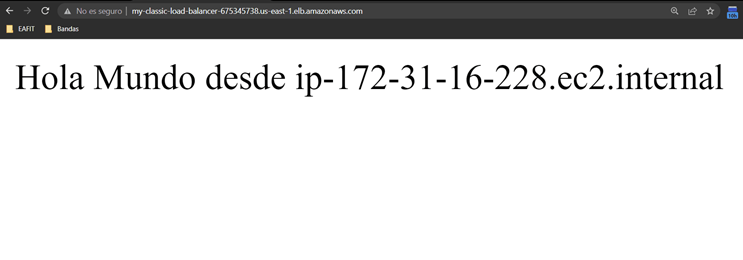
\includegraphics[width=\textwidth]{Figures/0. General/load_balancer_11.png}
        \caption{\textit{Las instancias cambian con cada request que realizmoas}}
        \label{fig: load balancer 11}
    \end{subfigure}
\end{figure}

\subsubsection{Compra del dominio}
Lo primero que se realizó fue la compra del dominio, una de las mejores ofertas
las ofrece \textit{Namecheap}, además de que el equipo ya contaba con cierta
experiencia con esta empresa. Los pasos realizados fueron:

\begin{itemize}
    \item Registro en la plataforma.
    \item Búsqueda del dominio deseado.
    \item Compra del dominio deseado.
    \item Configuración del dominio 
\end{itemize}

Ahora bien, los 3 primeros pasos son casi mecánicos para casis cualquier compra
en línea, pero ¿cómo realizamos el último paso? Bueno, lo primero que haremos es
ingresar a nuestro dominio y nos vamos a \textit{Configuración Avanzada}.

\begin{figure}[H]
    \centering
    \begin{subfigure}[b]{0.8\textwidth}
        \centering
        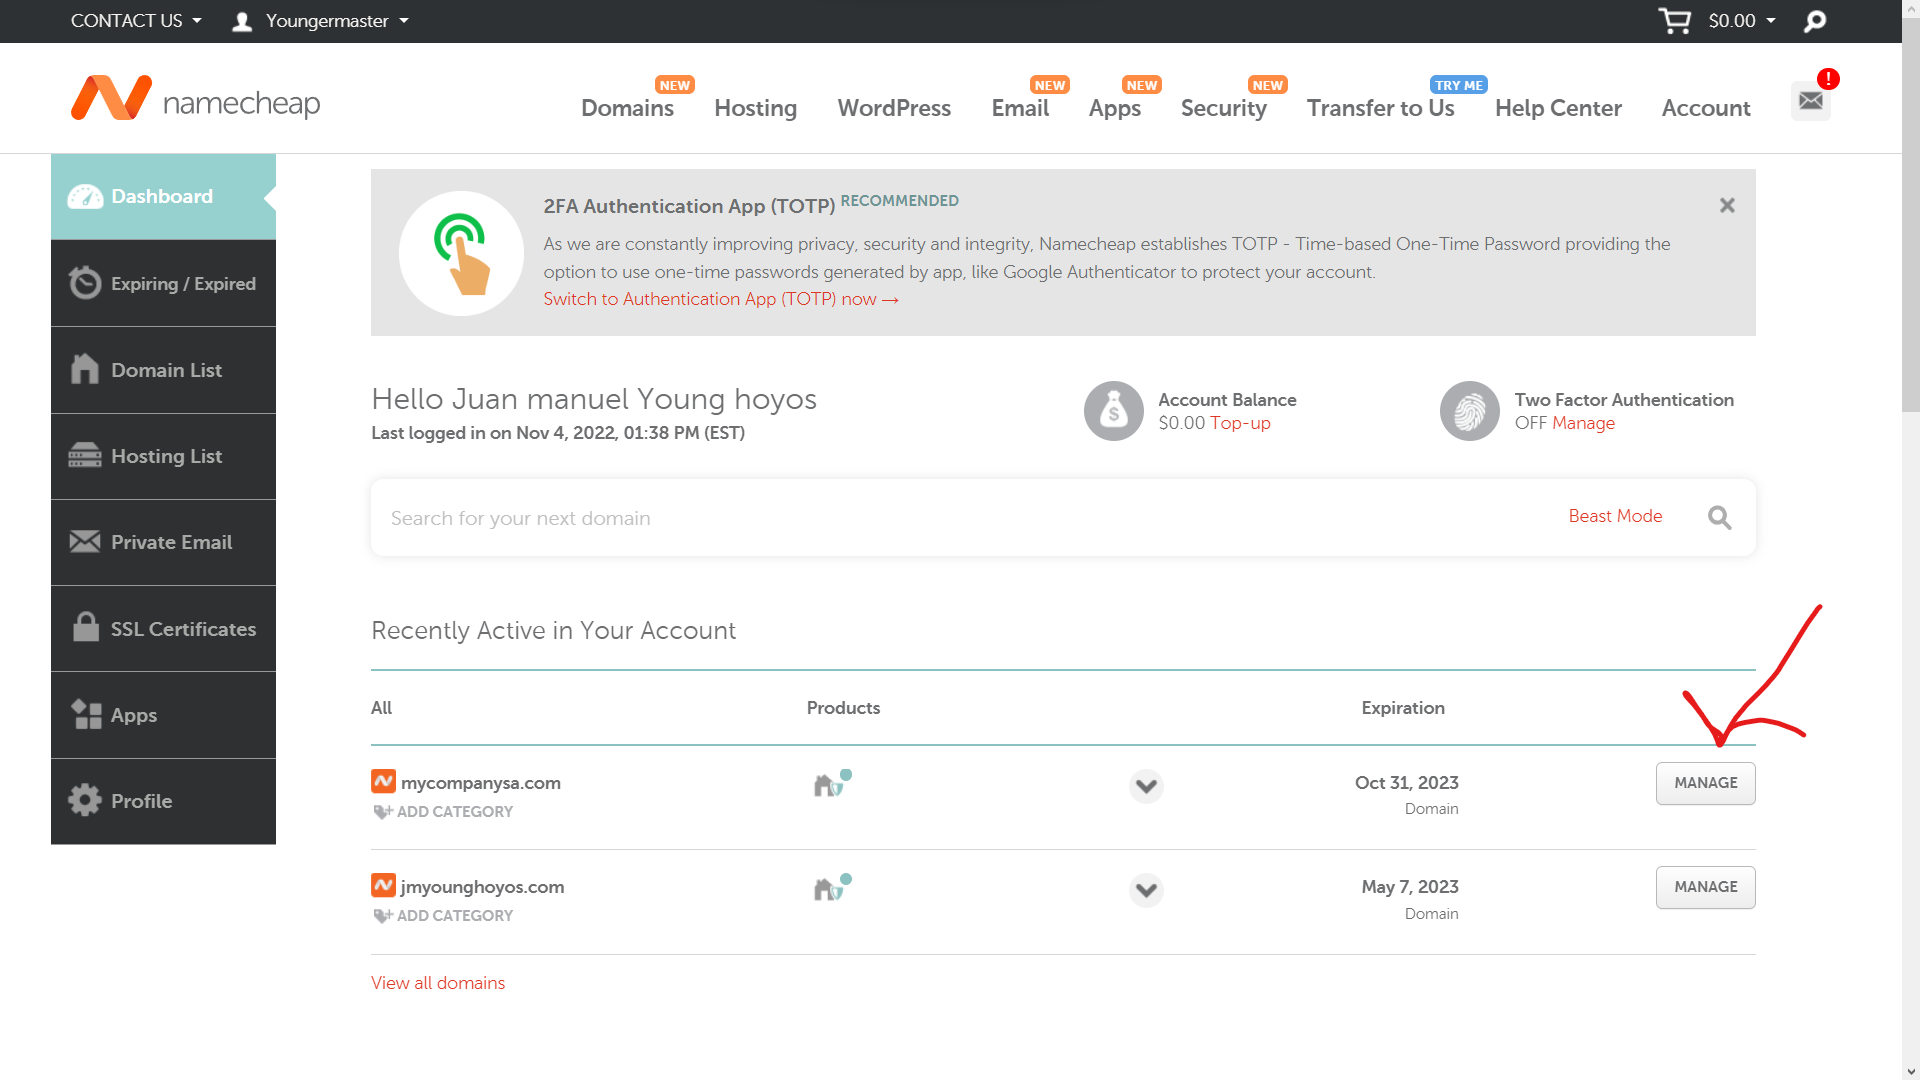
\includegraphics[width=\textwidth]{Figures/0. General/domain_selection.png}
        \caption{\textit{Selección del dominio}}
        \label{fig: domain selection}
    \end{subfigure}
\end{figure}

\begin{figure}[H]
    \centering
    \begin{subfigure}[b]{0.8\textwidth}
        \centering
        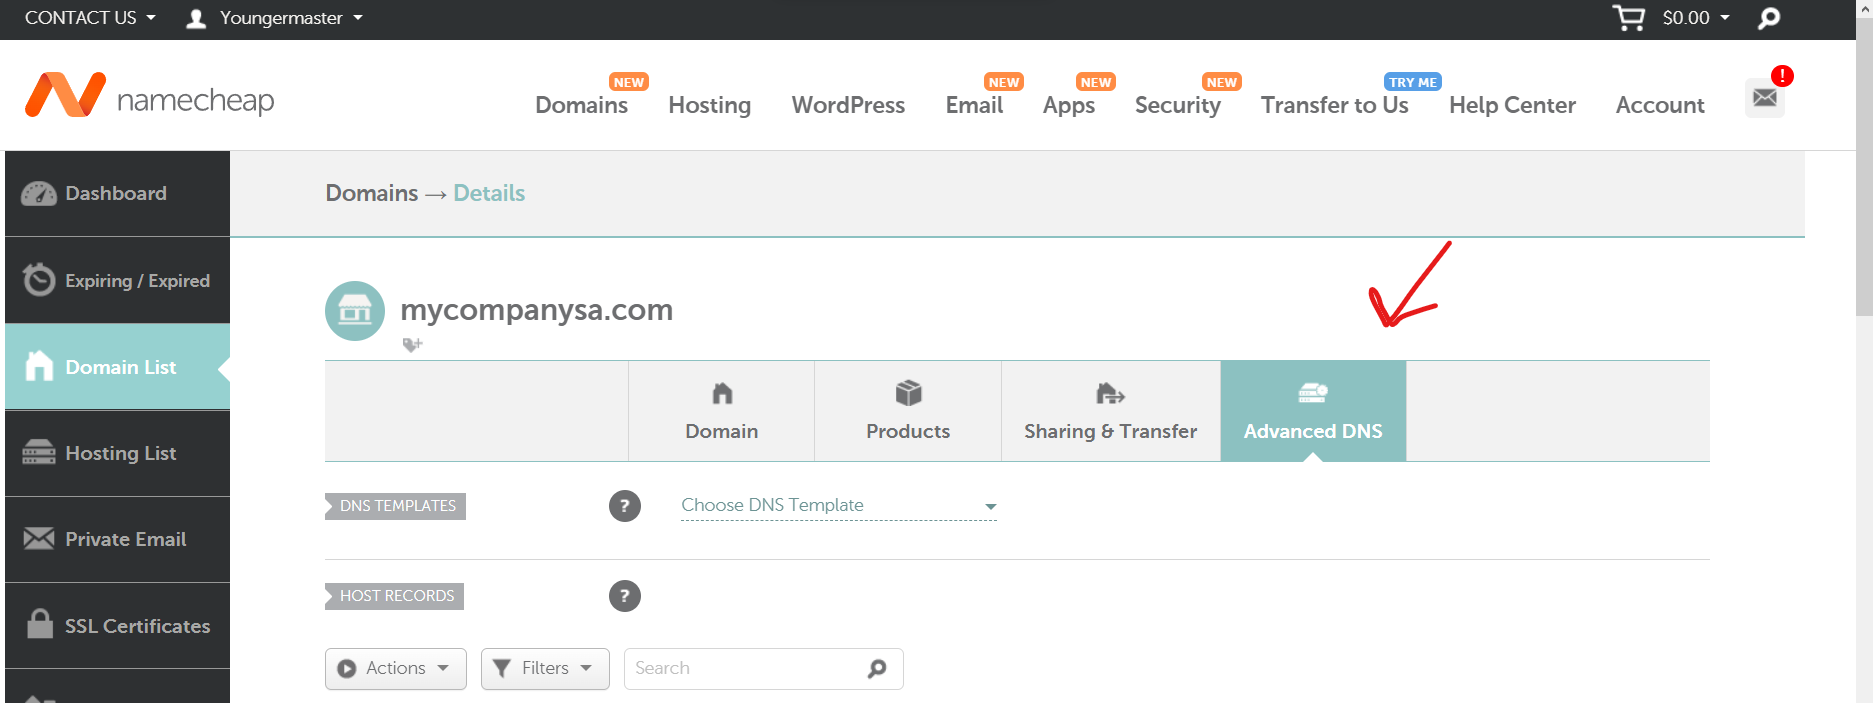
\includegraphics[width=\textwidth]{Figures/0. General/advanced_config_selection.png}
        \caption{\textit{Opción de configración avanzada de DNS}}
        \label{fig: advanced dns configuration}
    \end{subfigure}
\end{figure}

Después de esto añadiremos las siguientes rutas, los dominios e IPs son las
dadas por AWS, entonces se cambiarían las primeras IPs son reemplazadas por las
proporcionadas por el balanceador de cargas y los demás dominios hacen
referencia a lo que quieras desplegar en los diferentes dominios o subdominios.

\begin{figure}[H]
    \centering
    \begin{subfigure}[b]{0.8\textwidth}
        \centering
        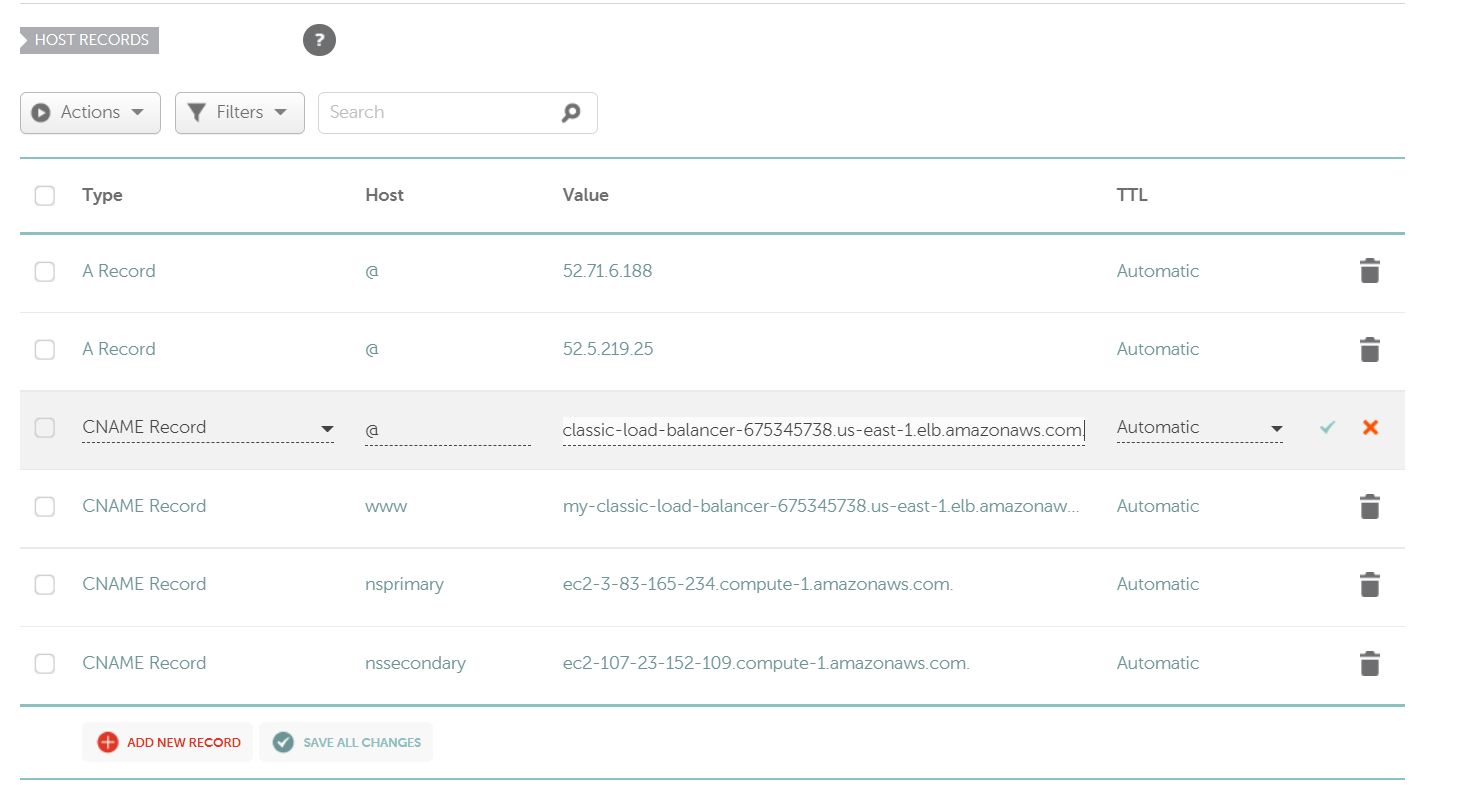
\includegraphics[width=\textwidth]{Figures/0. General/domain_config.png}
        \caption{\textit{Configración del dominio y subdominio en Namecheap}}
        \label{fig: domain configuration}
    \end{subfigure}
\end{figure}

\subsubsection{Configuración del aplicativo en cada dominio}

Primero realizmos el cambio a \textbf{\textit{\url{www.mycompanysa.com}}},
entonces tomamos las 3 primeras instancias que creamos, cuando accedemos
realizamos lo siguiente en la terminal.

\begin{lstlisting}[language=Bash]
curl -sL https://rpm.nodesource.com/setup_16.x | sudo bash -
sudo yum install git nodejs gcc-c++ make python3 docker -y
# * Services
sudo systemctl enable docker
sudo systemctl start docker
sudo systemctl stop httpd.service
# * Project setup
git clone https://github.com/Youngermaster/ST0255-2022-2-Projects.git
cd ST0255-2022-2-Projects/project-2/MyCompanySA
sudo docker build -t mycompanysa:release .
sudo docker run -d -it -p 80:8000 mycompanysa:release
\end{lstlisting}

Al realizarlo en los 3 nodos si accedemos a 
\textbf{\textit{\url{www.mycompanysa.com}}} esto nos devolverá el siguiente
aplicativo, donde podremos escribir y leer reviews de diferentes productos:

\begin{figure}[H]
    \centering
    \begin{subfigure}[b]{0.8\textwidth}
        \centering
        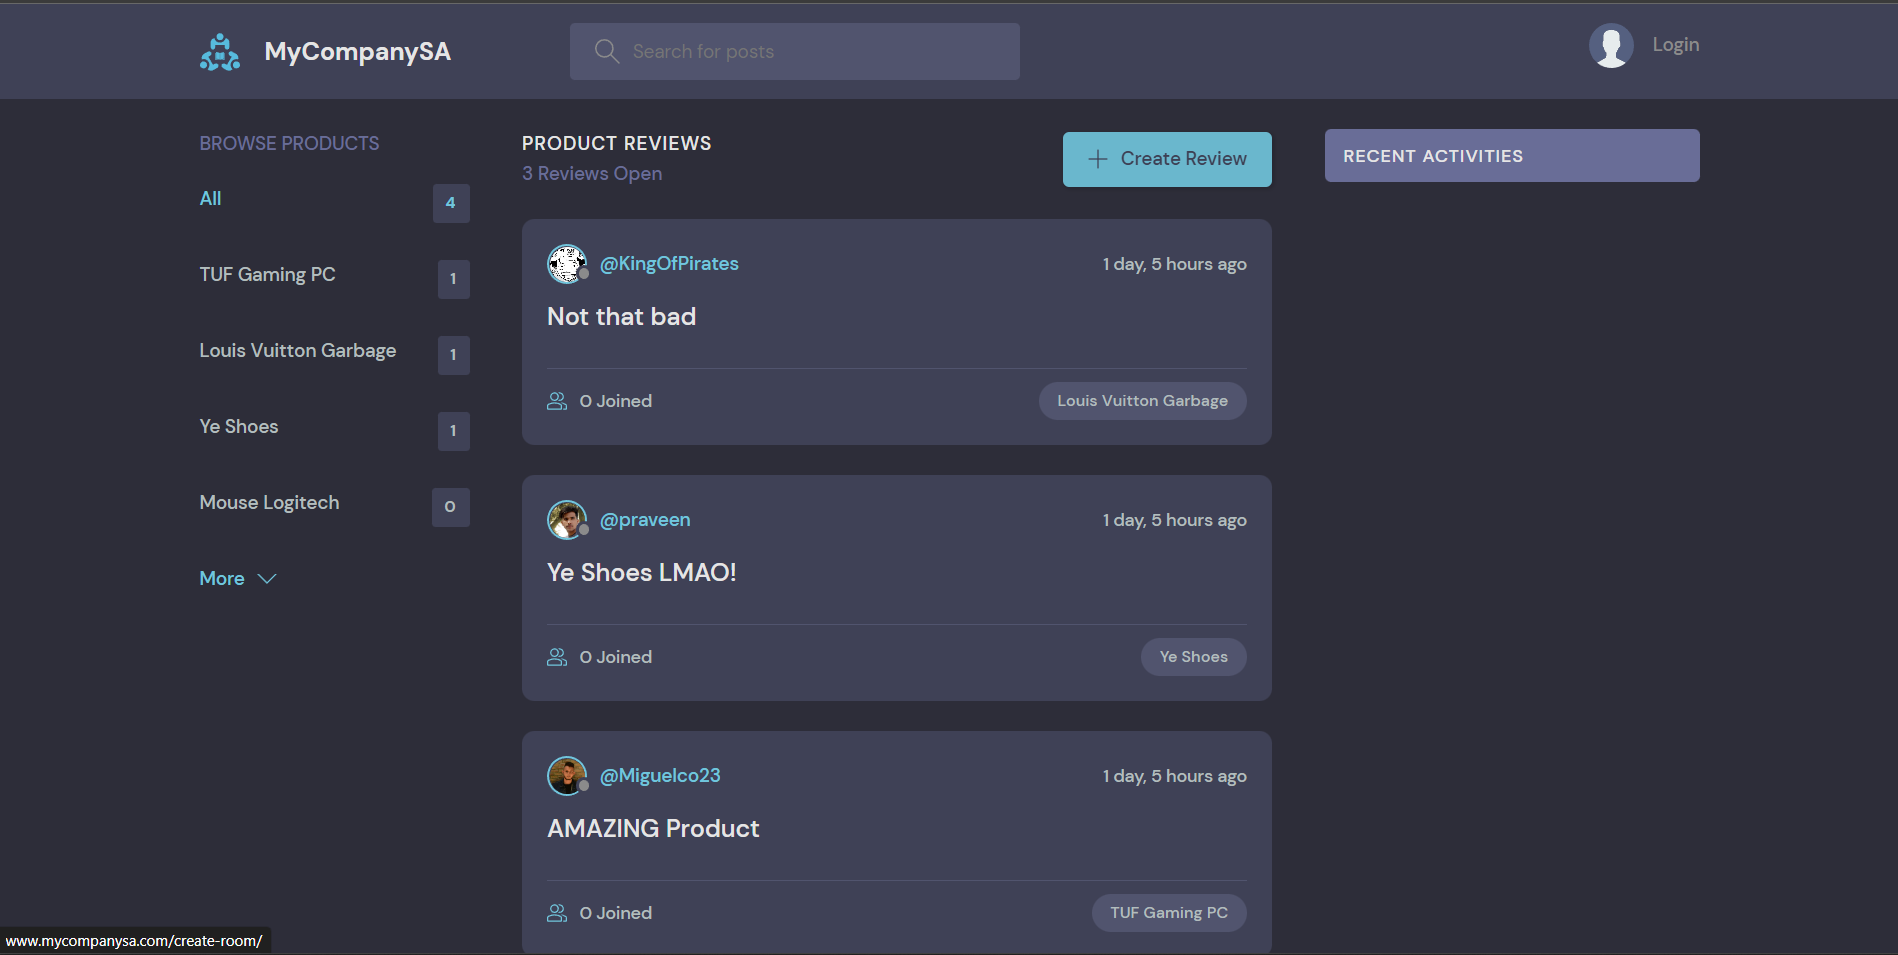
\includegraphics[width=\textwidth]{Figures/0. General/www.mycompanysa.com.png}
        \caption{\textbf{\textit{\url{www.mycompanysa.com}}}}
        \label{fig: www.mycompanysa.com config}
    \end{subfigure}
\end{figure}

Ahora si creamos una instancia de EC2 para el subdominio
\textbf{\textit{\url{nsprimary.mycompanysa.com}}}, entramos a través de SSH e
ingresamos lo siguiente y obtendremos una landing page:

\begin{lstlisting}[language=Bash]
curl -sL https://rpm.nodesource.com/setup_16.x | sudo bash -
sudo yum install git nodejs gcc-c++ make python3 docker -y
# * Services
sudo systemctl enable docker
sudo systemctl start docker
sudo systemctl stop httpd.service
# * Project setup
git clone https://github.com/Youngermaster/ST0255-2022-2-Projects.git
cd ST0255-2022-2-Projects/project-2/nsprimary
docker build -t nsprimary-mycompanysa:release .
docker run -d -it -p 80:8000 nsprimary-mycompanysa:release
\end{lstlisting}

\begin{figure}[H]
    \centering
    \begin{subfigure}[b]{0.8\textwidth}
        \centering
        
\includegraphics[width=\textwidth]{Figures/0. General/nsprimary.mycompanysa.com.png}
        \caption{\textbf{\textit{\url{nsprimary.mycompanysa.com}}}}
        \label{fig: nsprimary.mycompanysa.com config}
    \end{subfigure}
\end{figure}


Ahora si creamos una instancia de EC2 para el subdominio
\textbf{\textit{\url{nssecondary.mycompanysa.com}}}, entramos a través de SSH e
ingresamos lo siguiente y obtendremos una Blog para MyCompanySA:

\begin{lstlisting}[language=Bash]
curl -sL https://rpm.nodesource.com/setup_16.x | sudo bash -
sudo yum install git nodejs gcc-c++ make python3 docker -y
# * Services
sudo systemctl enable docker
sudo systemctl start docker
sudo systemctl stop httpd.service
# * Project setup
git clone https://github.com/Youngermaster/ST0255-2022-2-Projects.git
cd ST0255-2022-2-Projects/project-2/nssecondary
docker build -t nssecondary-mycompanysa:release .
docker run -d -it -p 80:80 nssecondary-mycompanysa:release
\end{lstlisting}

\begin{figure}[H]
    \centering
    \begin{subfigure}[b]{0.8\textwidth}
        \centering
        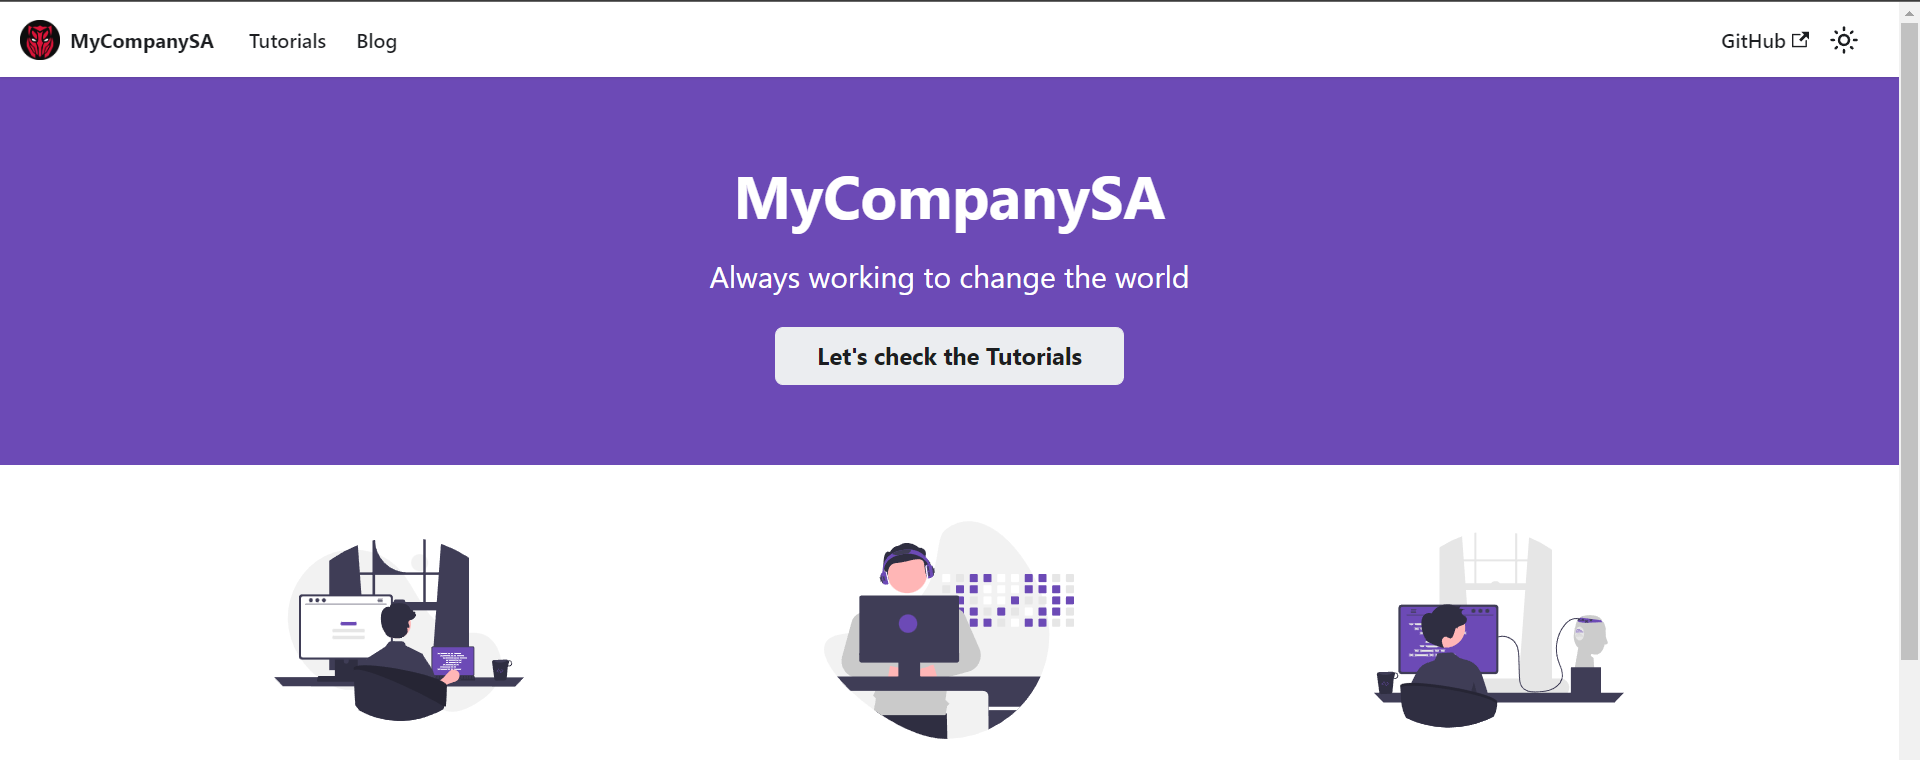
\includegraphics[width=\textwidth]{Figures/0. General/nssecondary.mycompanysa.com.png}
        \caption{\textbf{\textit{\url{nssecondary.mycompanysa.com}}}}
        \label{fig: nssecondary.mycompanysa.com config}
    \end{subfigure}
\end{figure}

\subsection{Disponibilidad para miles de usuarios}
Ahora bien, como se mencionó al principio, lo más importante es una alta
disponibilidad, entonces probemos $1000$, $1500$ y $3000$ usuarios concurrentes 
para ver el comportamiento. Para esto usaremos \textbf{\textit{\url{locust}}}.\\

En nuestra máquina lanzamos lo siguiente, pero hay que estar seguros que estemos
en la carpeta del proyecto.

\begin{lstlisting}[language=Bash]
cd project-1/Load-Testing
# Primero con 1000
locust -f locust.py --host http://www.mycompanysa.com/ --users 1000 --spawn-rate 20
# Luego con 1500
locust -f locust.py --host http://www.mycompanysa.com/ --users 1500 --spawn-rate 20
# Luego con 3000
locust -f locust.py --host http://www.mycompanysa.com/ --users 3000 --spawn-rate 20
\end{lstlisting}

Obtendremos la siguiente interfaz y le damos en el botón de empezar:

\begin{figure}[H]
    \centering
    \begin{subfigure}[b]{0.8\textwidth}
        \centering
        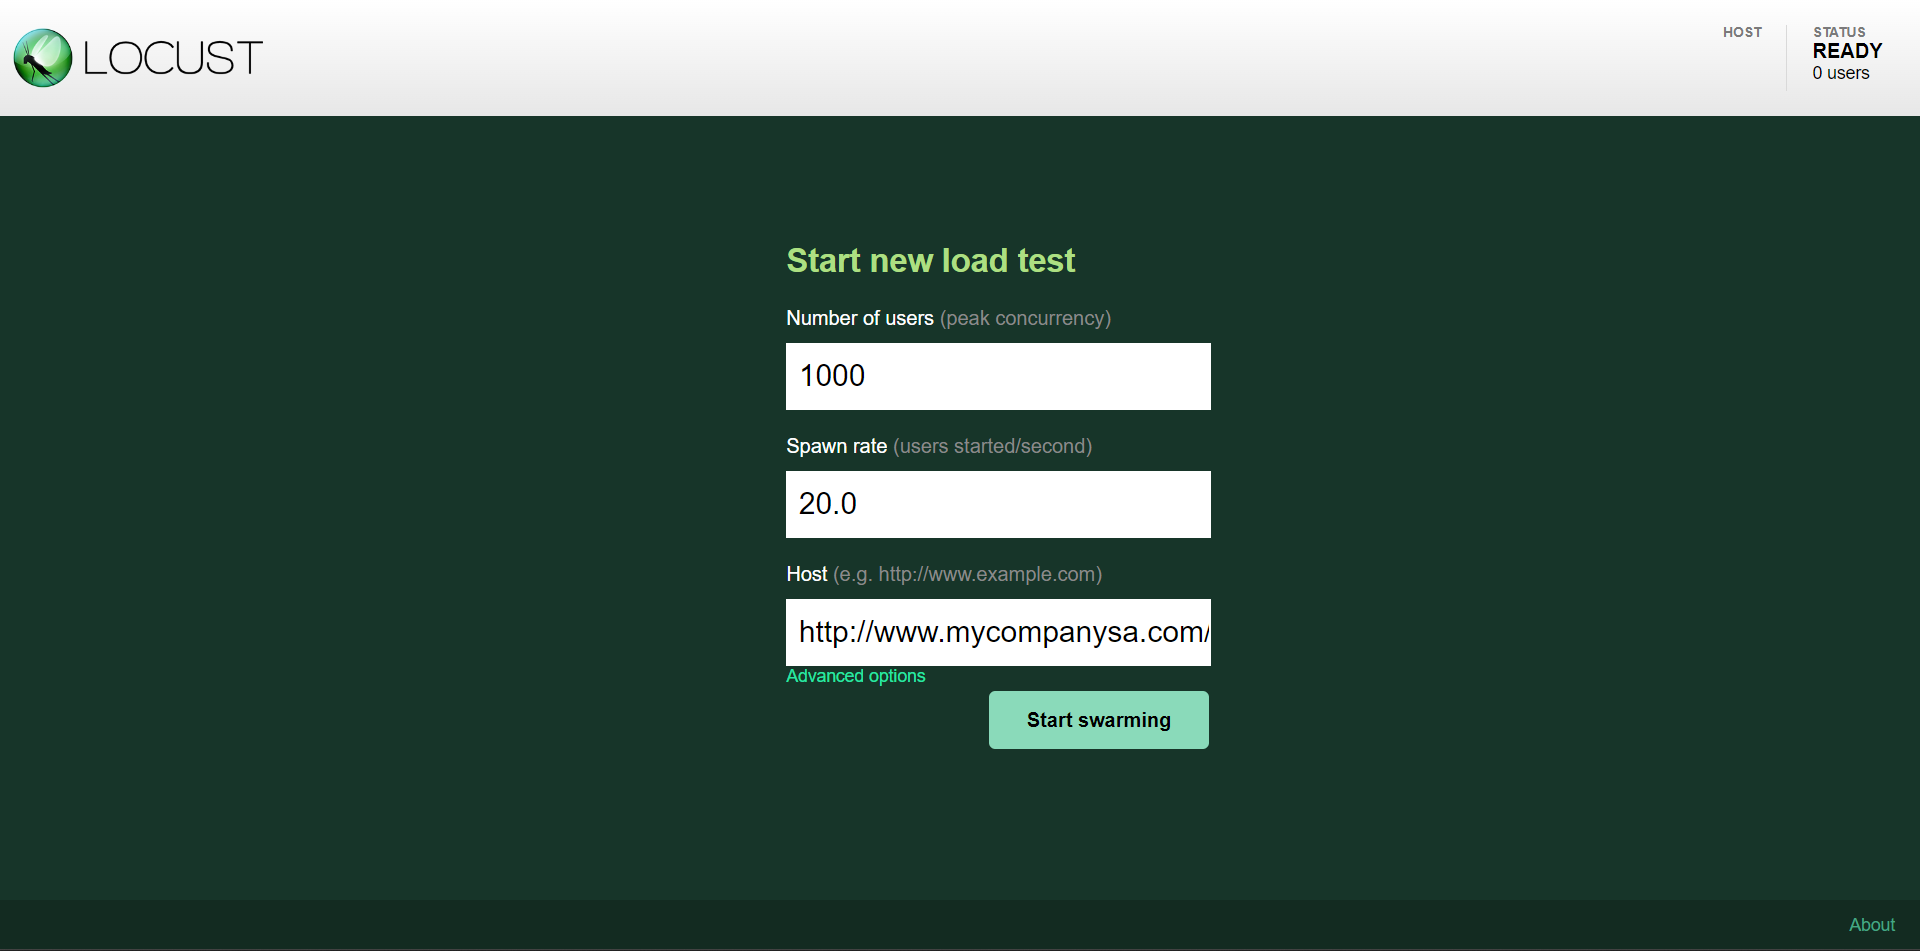
\includegraphics[width=\textwidth]{Figures/0. General/locust_0.png}
        \caption{\textbf{Locust configuración}}
        \label{fig: Locust config}
    \end{subfigure}
\end{figure}

Un ejemplo de cómo se ve la interfaz es la siguiente:

\begin{figure}[H]
    \centering
    \begin{subfigure}[b]{0.8\textwidth}
        \centering
        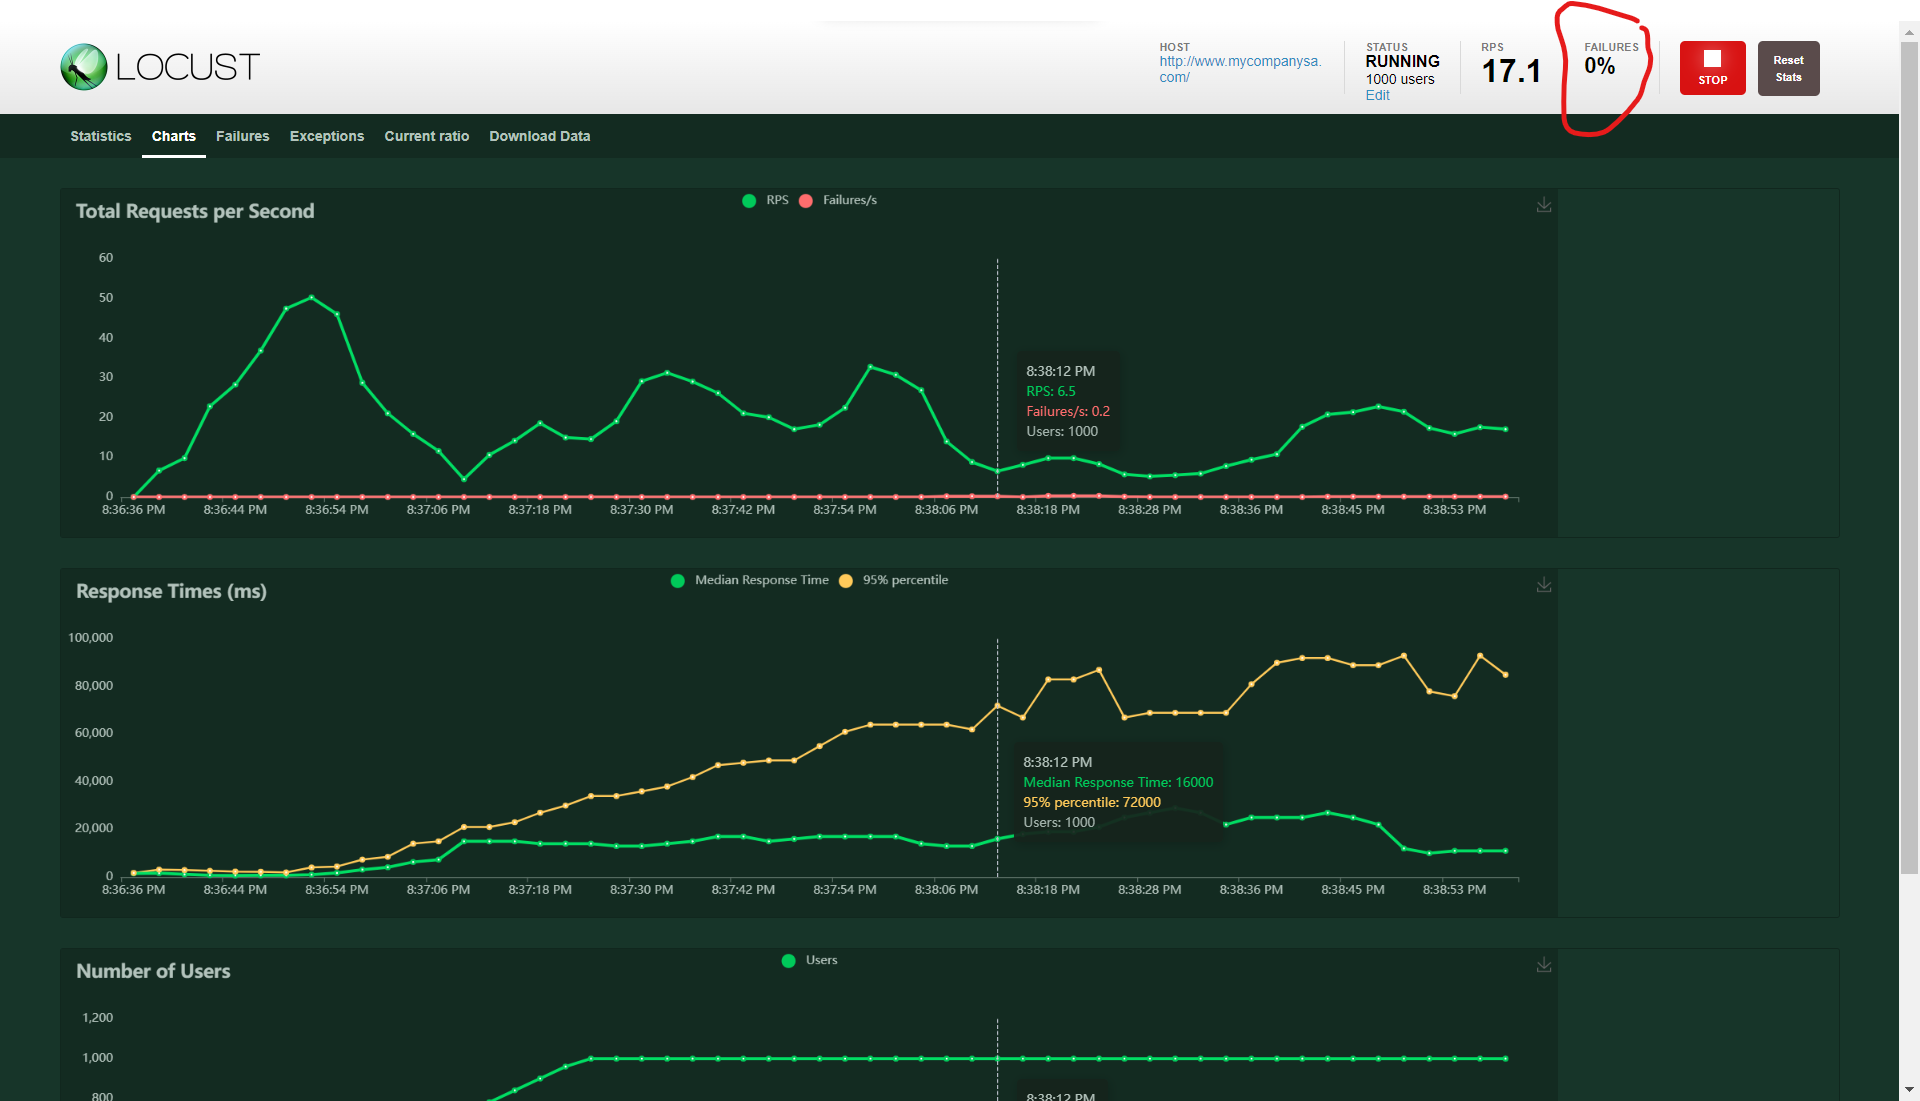
\includegraphics[width=\textwidth]{Figures/0. General/locust_1000.png}
        \caption{\textbf{Locust $1000$}}
        \label{fig: Locust 1000}
    \end{subfigure}
\end{figure}

En conclusión is revisamos a fondo después de realizar las pruebas obtendremos
que la mayor cantidad de usuarios soportados concurrentemente es de $1840$.

\subsection{Demo}
Las direcciónes para probar el despliegue son:

\begin{itemize}
    \item \textbf{\textit{\url{www.mycompanysa.com}}}
    \item \textbf{\textit{\url{nsprimary.mycompanysa.com}}}
    \item \textbf{\textit{\url{nssecondary.mycompanysa.com}}}
\end{itemize}